\section{Performance Evaluation}\label{performanceEvaluation}

We present in this section metrics that are useful to evaluate the experimental results shown in the previous section.

\subsection{Total benchmark execution times}\label{summaryTotalTimes}

We provide first in Figure \ref{fig:totalTimesSummary} a summary of the total benchmark execution times for the various configurations. The best overall time corresponds to Databricks using statistics and data partitioning. Among the other systems, EMR Spark obtains the best time when using data partitioning and the optimizer disabled by default. Databricks Light obtains similar times to EMR Spark, but we remark that we did not test data partitioning for this system. The best time with EMR Presto is obtained by using statistics, but even with the resulting improvement the system ends up ranking last.

\begin{figure}
   \begin{center}
   \scalebox{0.70}{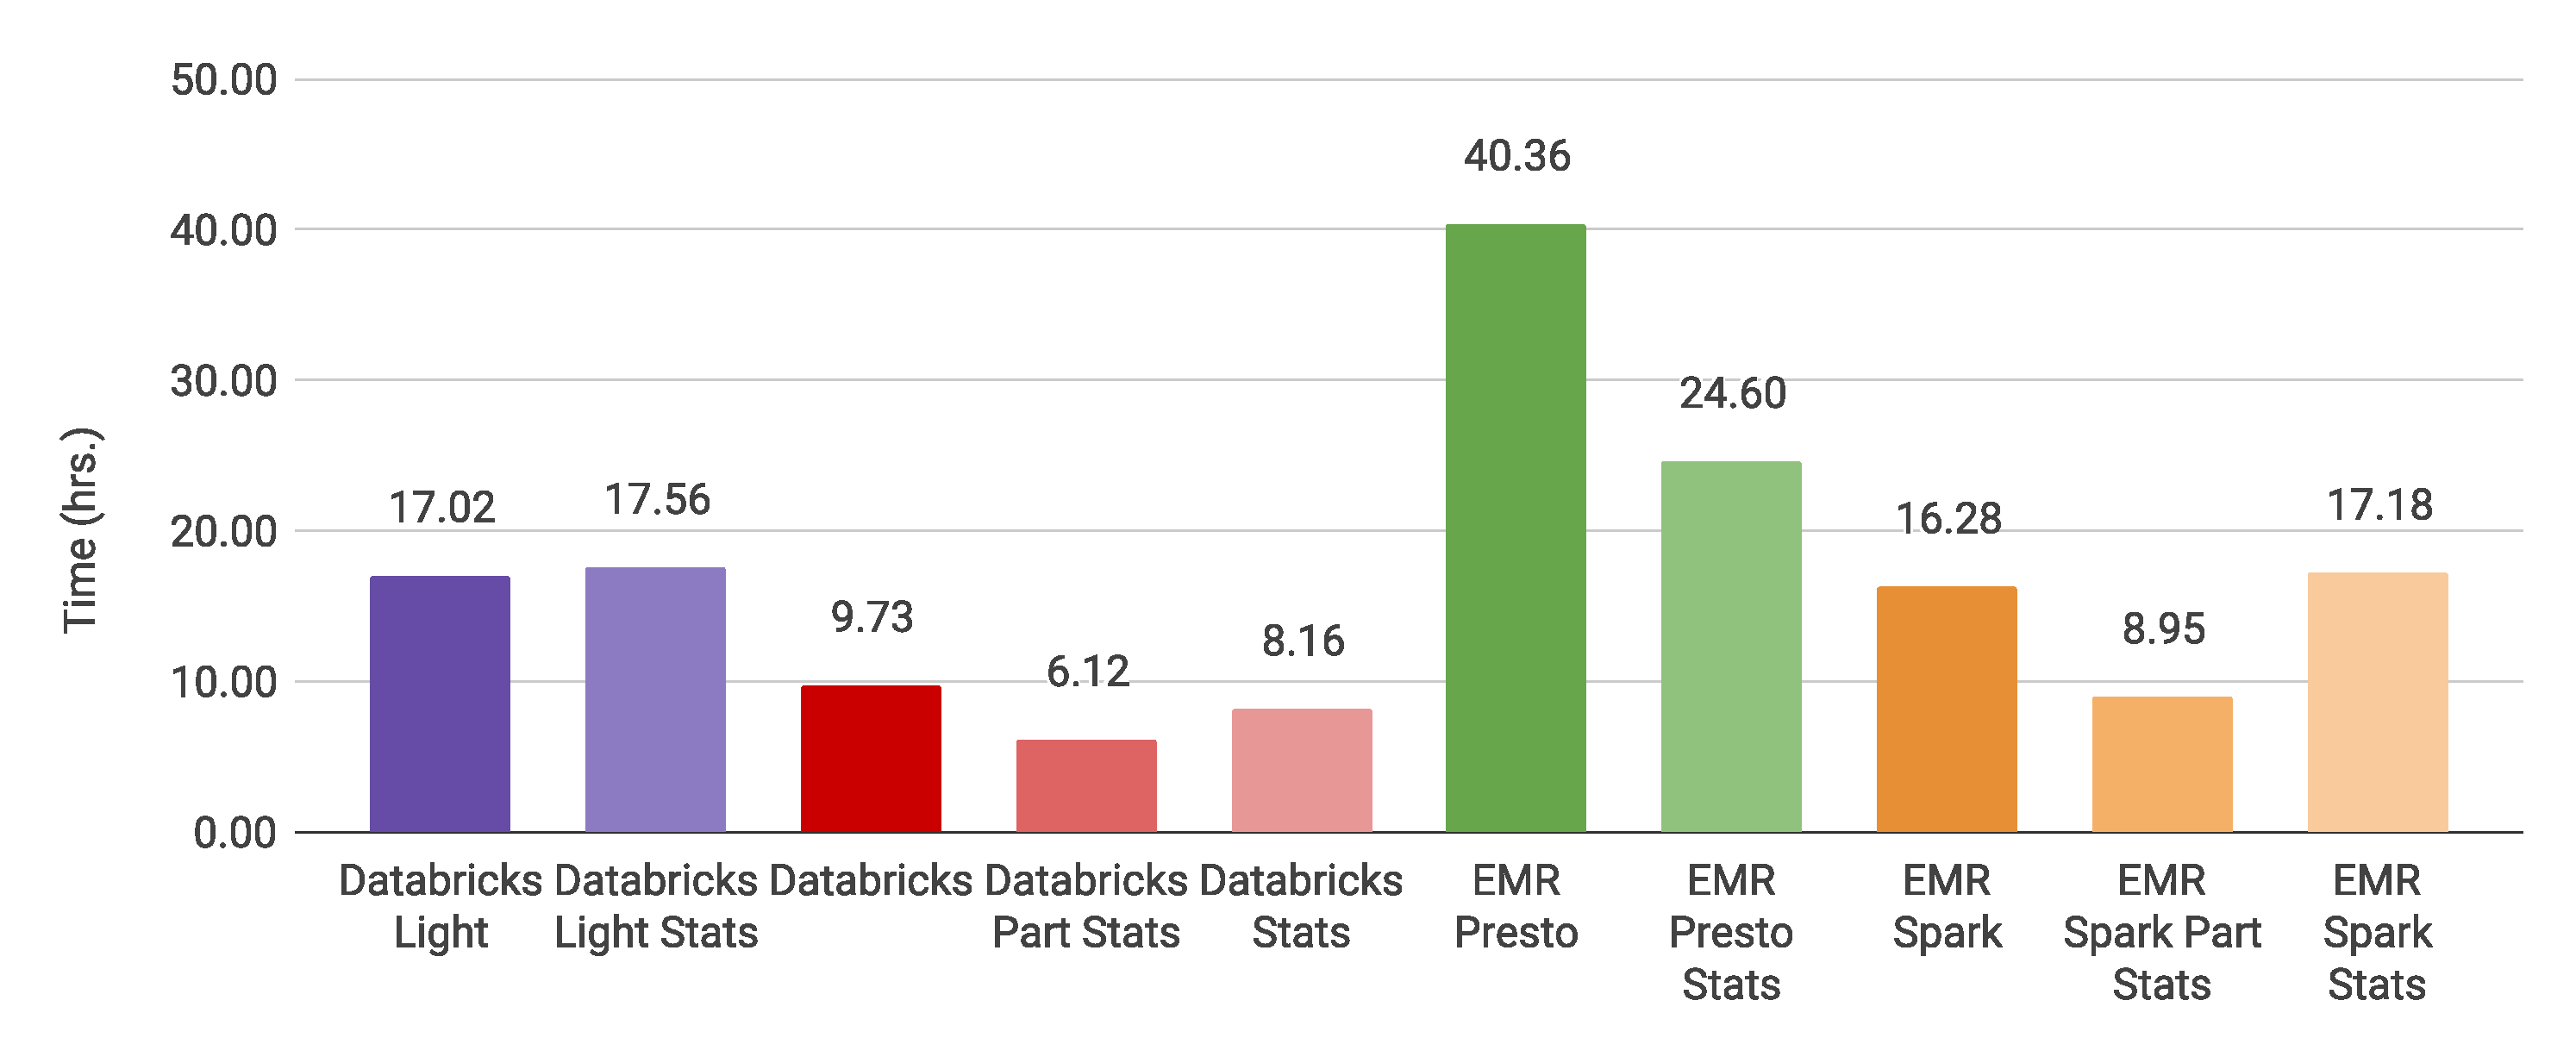
\includegraphics[width=7.0in]{imgs/totalTimesSummary.pdf}}
   \end{center}
   \caption{Summary of total execution times for the TPC-DS benchmark at the 1 TB scale factor.}
   \label{fig:totalTimesSummary}
\end{figure}

\subsection{TPC Benchmark DS Metric}\label{summaryTpcdsMetric}

The TPC Benchmark DS defines a performance metric calculated from the execution times of the individual tests (Data Loading, Power, and Throughput). We present in Figure \ref{fig:tpcdsMetricSummary} the results for this metric for the various SUTs, in this case higher values are better. The details of the calculation of the metric can be found in \cite{tpcdsSpec}.

\begin{figure}
   \begin{center}
   \scalebox{0.70}{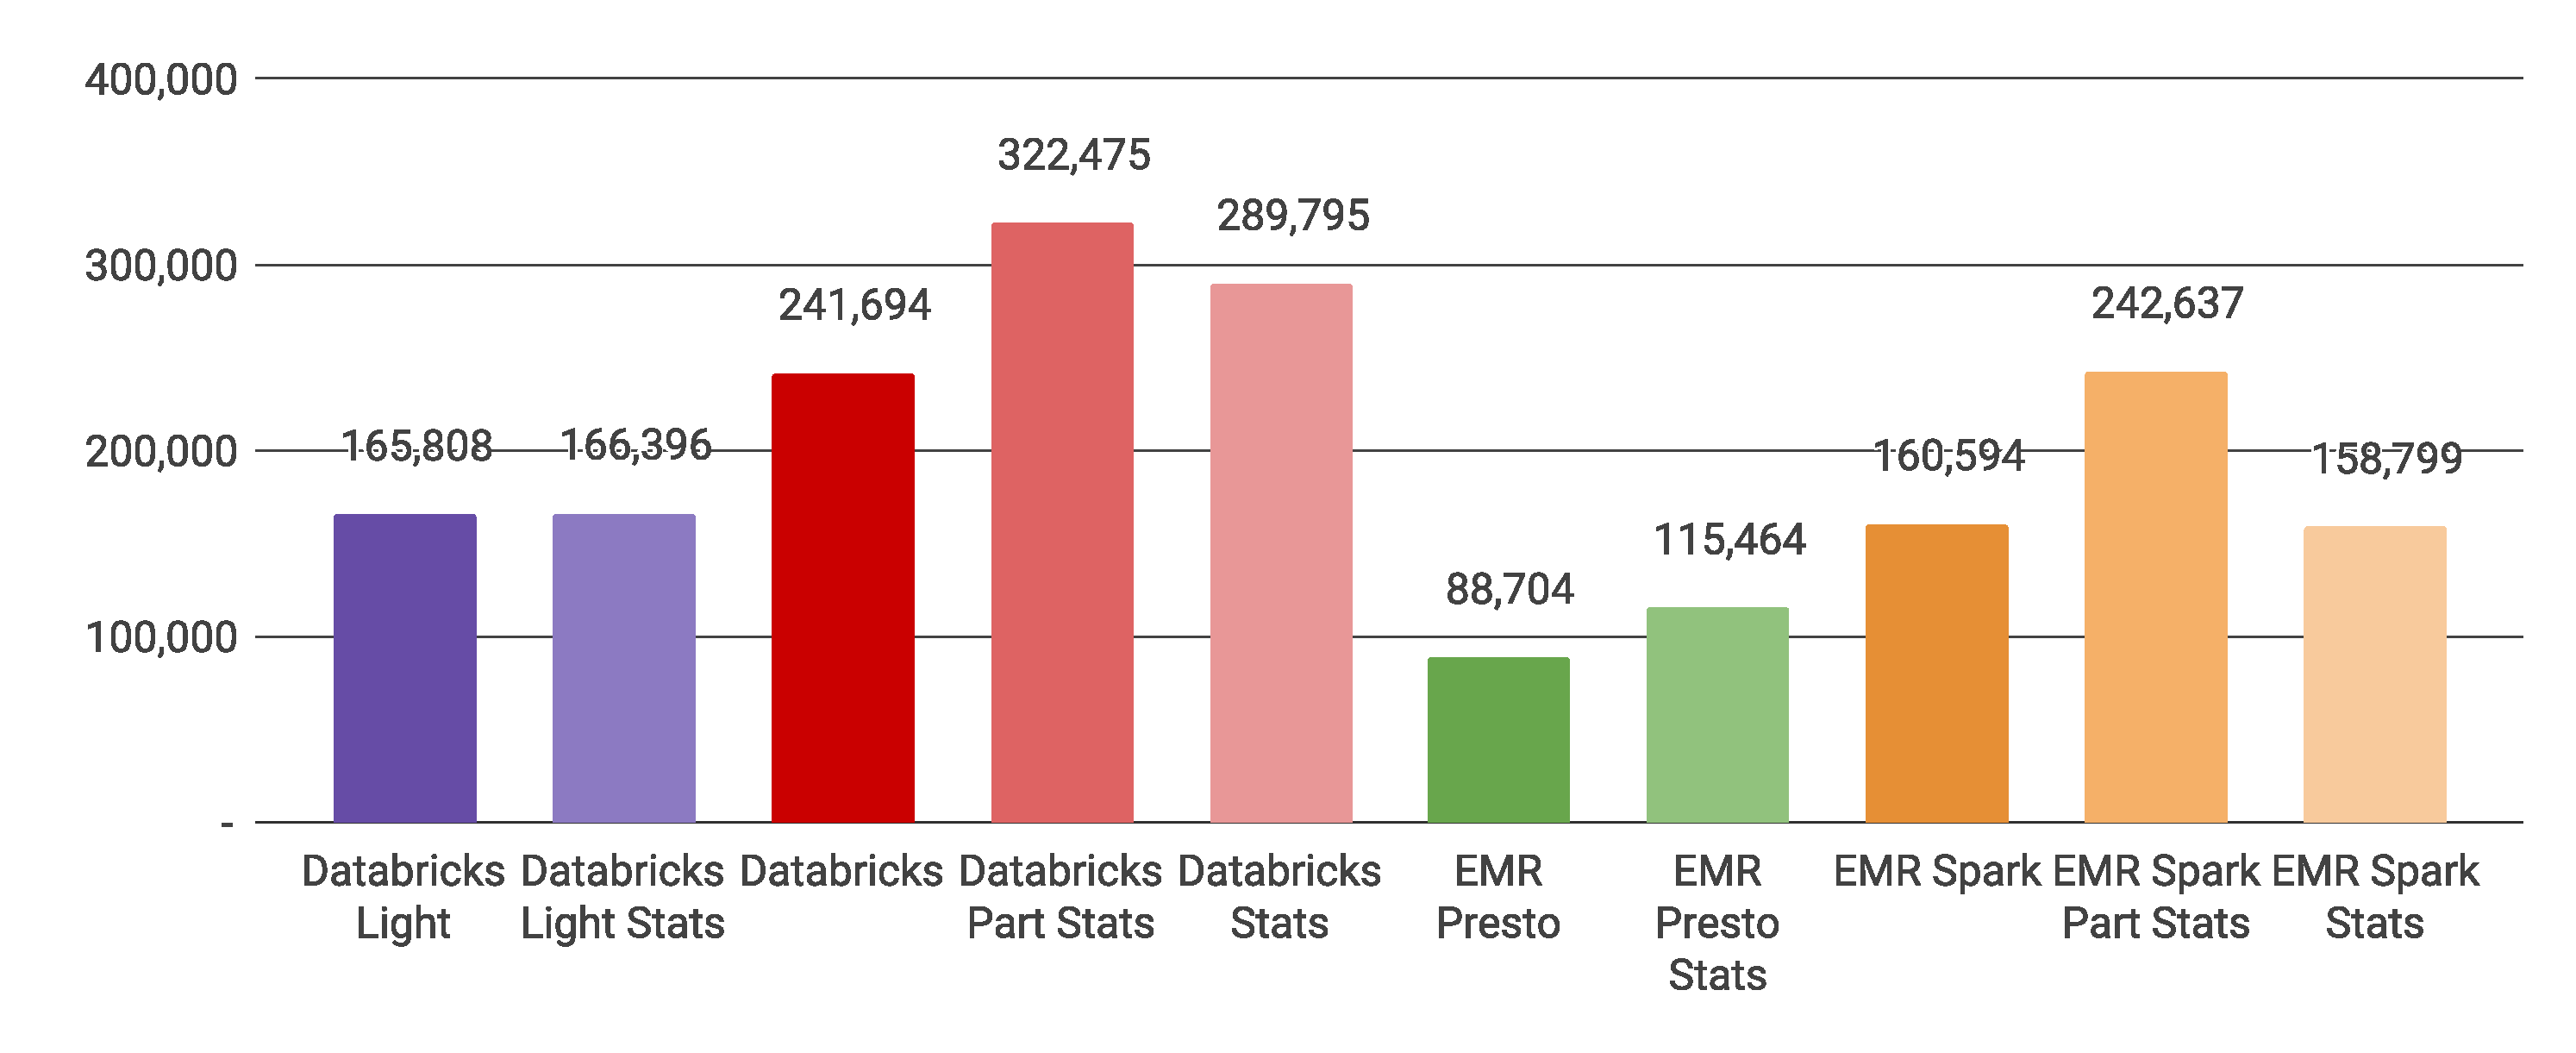
\includegraphics[width=7.0in]{imgs/tpcdsMetricSummary.pdf}}
   \end{center}
   \caption{Summary of total execution times for the TPC-DS benchmark at the 1 TB scale factor.}
   \label{fig:tpcdsMetricSummary}
\end{figure}

The scores for the TPC-DS benchmark essentially reflect the benchmark total execution times. Again the best result is achieved by Databricks using statistics and data partitioning. The next best result corresponds to EMR Spark while EMR Presto obtains the lowest scores and rank.

\subsection{TPC Benchmark DS Metric}\label{summaryTpcdsMetric}

In order to select the best option for cloud-based big data analytics performance metrics based on query evaluation times are very useful but insufficient. It is essential for organizations to also take into consideration the monetary costs associated with those performance results. In the adoption of a cloud-based system there usually separate costs for hardware and software use. This is the case for the systems we consider in this report and these costs are summarized in Table \ref{table:systemCosts}.

\begin{table}
  \centering
	\begin{tabular}{|l|l|l|}
	  \hline
		\textbf{System} & \textbf{Hardware} & \textbf{Software} \\ \hline
		EMR Presto & \$0.0624 & \$0.156 \\ \hline
		EMR Spark & \$0.0624 & \$0.156 \\ \hline
		Databricks & \$0.0624 & \$0.3 \\ \hline 
		Databricks Light & \$0.0624 & \$0.14 \\ \hline 
	\end{tabular}
	\caption{Per-node per-hour hardware and software costs of the SUTs.}
	\label{table:systemCosts}
\end{table}

We exclude in this report the AWS S3 storage costs as well as the costs involved in development and testing. The total cost of executing the TPC-DS benchmark is then calculated by the sum of the hardware and software costs per-node (Table \ref{table:systemCosts}) multiplied by the number of nodes (9 in all cases counting the master node) and then multiplied by the total execution time (in hours). These calculations yield the costs presented in Figure \ref{fig:totalCostsSummary}.

\begin{figure}
   \begin{center}
   \scalebox{0.70}{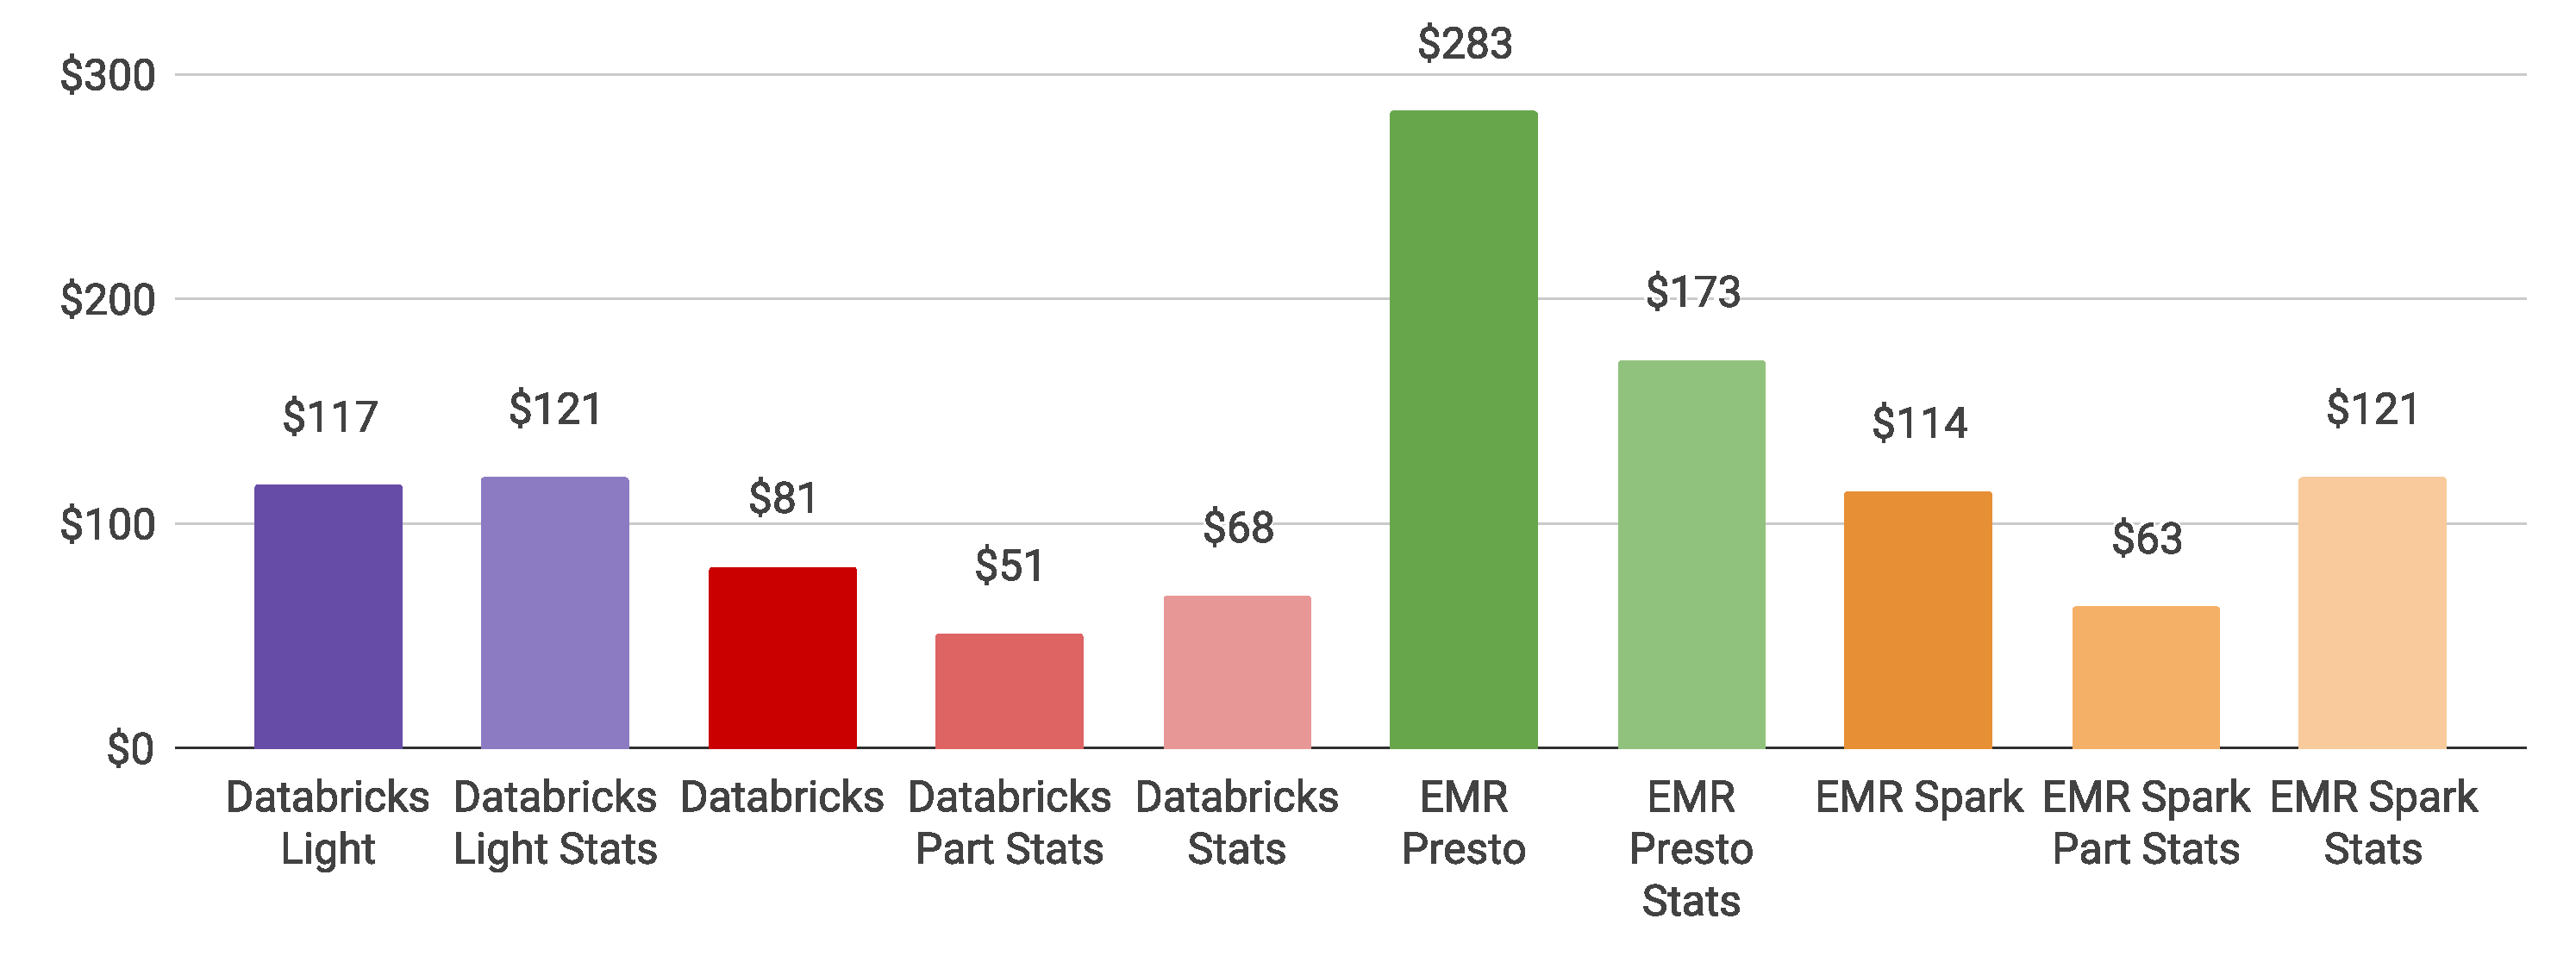
\includegraphics[width=7.0in]{imgs/totalCostsSummary.pdf}}
   \end{center}
   \caption{Summary of total costs for the TPC-DS benchmark at the 1 TB scale factor.}
   \label{fig:totalCostsSummary}
\end{figure}

The lowest cost overall is achieved by Databricks using statistics and data partitioning at \$51. It is noteworthy that Databricks obtains the lowest cost despite higher costs per-node per-hour. The next best result (\$63) puts EMR Spark at the second place and is obtained using data partitioning. The best cost for EMR Presto (\$173) is over three times higher than the best cost for Databricks and higher than the costs for Databricks Light.

Given the TPC-DS metric results and the associated costs incurred to achieve them we can derive a single price-performance metric to compare the various systems. The results for this price-performance metric are presented in Figure \ref{fig:pricePerformanceSummary}, in this case smaller values are better. Essentially, the price-performance results are congruent to the monetary costs, favoring Databricks with statistics and data partitioning. EMR Spark, Databricks Light and EMR Presto are next in the ranking.

\begin{figure}
   \begin{center}
   \scalebox{0.70}{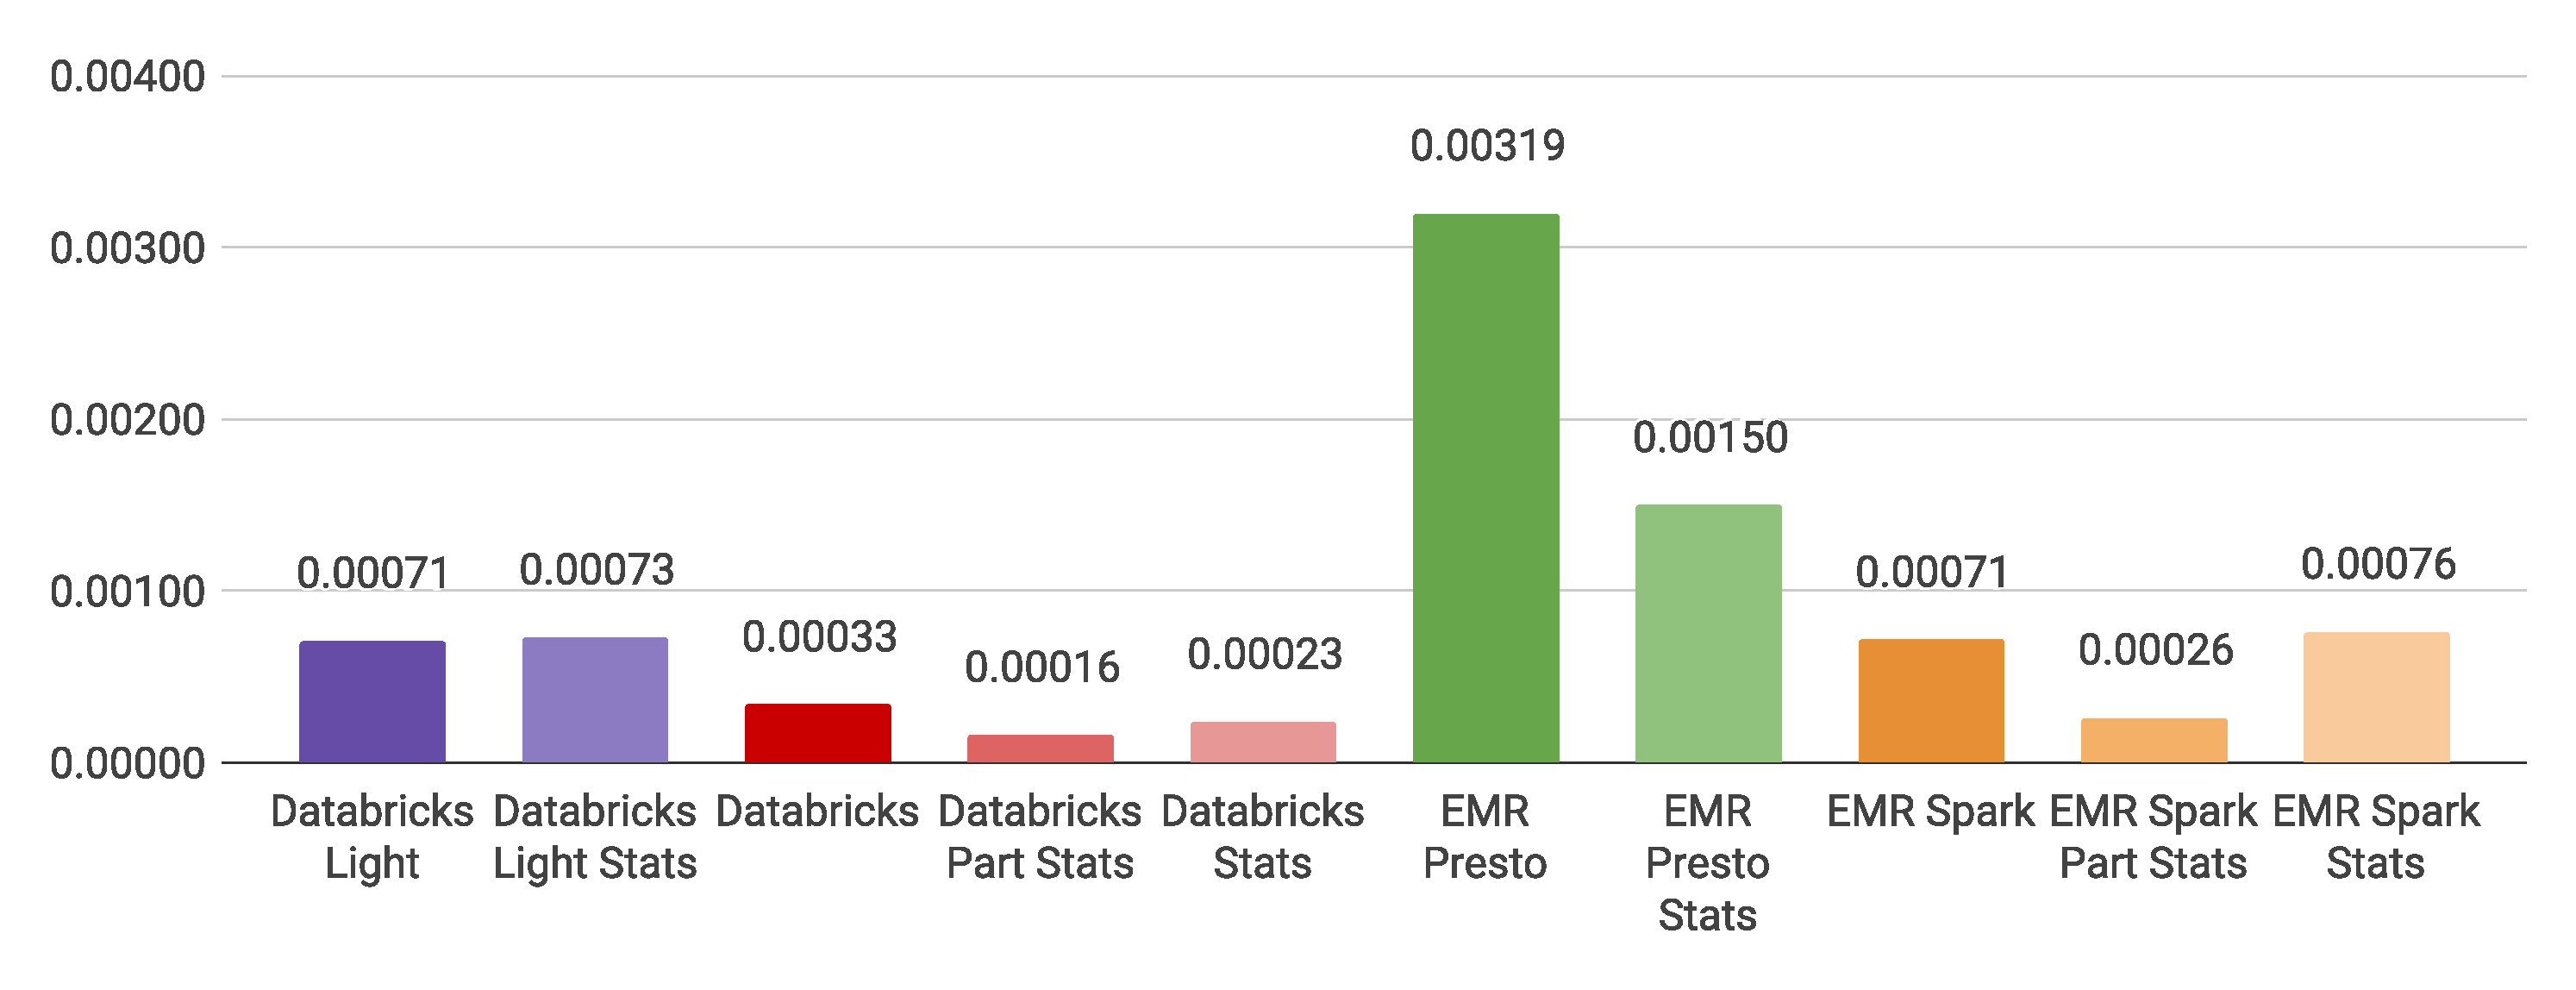
\includegraphics[width=7.0in]{imgs/pricePerformanceSummary.pdf}}
   \end{center}
   \caption{Summary of price-performance for the TPC-DS benchmark at the 1 TB scale factor.}
   \label{fig:pricePerformanceSummary}
\end{figure}










